\documentclass[12pt]{article}
\usepackage{amsmath}
\usepackage{amssymb}
\usepackage{geometry}
\usepackage{enumerate}
\usepackage{natbib}
\usepackage{float}%稳定图片位置
\usepackage{graphicx}%画图
\usepackage[english]{babel}
\usepackage{a4wide}
\usepackage{indentfirst}%缩进
\usepackage{enumerate}%加序号
\usepackage{multirow}%合并行
\title{\large UM-SJTU JOINT INSTITUTE\\PHYSICS LABORATORY\\(VP141)\\\ \\\ \\\ \\\ \\\ \\\ \\\ \\\ \\\ \\\ \\\
LABORATORY REPORT\\\ \\\ EXERCISE 3\\\  SIMPLE HARMONIC MOTION\\OSCILLATIONS IN MECHANICAL SYSTEMS \\\ \\\ \\\ \\\ \\\ }
\author{Name: Pan Chongdan\\ID: 516370910121\\Partner: Yang Ruiming\\ID:516370910127\\Group: 16}
\date{Date: \today}

\begin{document}
\maketitle
\newpage
\section{Objectives}
In this exercise I'll study simple harmonic motion and learn how to use air track to find the spring constant and effective mass of a spring. I'll also analyse the relationship between the oscillation period and the mass of the oscillator, check whether the oscillation period depends on the the amplitude, and examine the relationship between the maximum speed and the amplitude.
\section{Theoretical Background} 
\subsection{Basic Concept of Simple Harmonic Motion}
There are various kinds of periodic motion in nature.The simple harmonic motion is the simplest and most fundamental, where the restoring force is proportional to the displacement from the equilibrium position and as a result, the position of a particle depends on time as the sine or cosine function. Discussion of the simple harmonic motion is a basis for studying more complex situations.
\subsubsection{Hooke's Law}
Within the elastic limit of deformation, the force $F_x$ needed to be applied in order to stretch or compress a spring by the distance x is proportional to that distance,for example:
\begin{equation}
F_x=kx
\end{equation}
where k is a constant (called the spring constant) characterizing how easy it is to deform the spring. This constant will be found in the present exercise using a measurement device called the \emph{Jolly balance}. The linear relation (1), between the force and the deformation, is known as the \emph{Hooke's Law}. According to Newton's third law of dynamics, the spring exerts a reaction elastic force of the same magnitude but opposite direction. As this force tries to restore the system back to the equilibrium, it is also known as the restoring force.
\subsubsection{Equation of Motion of the Simple Harmonic Oscillator}
\begin{figure}[H]
\centering
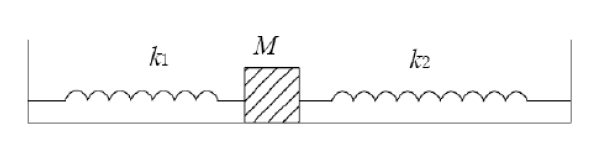
\includegraphics[]{P1.jpg}
\caption{Mass-spring system}
\end{figure}
As shown in Figure 1, an object with mass M is set on an air track with a spring
attached to both of its sides. The purpose of using the air track is to eliminate frictional forces between moving surfaces. The other ends of the springs are fixed to the air track.The spring constants $k_1$ and $k_2$ are to be measured with the Jolly balance. The origin $(x=0)$ of the coordinate system is set at the equilibrium position of the mass $M$.Assuming that the masses of the springs can be ignored, and neglecting damping in the system, the elastic (restoring) forces of the springs are the only forces acting on mass $M$. According to Newton's second law of dynamics, the equation of motion of mass $M$ is
\begin{equation}
M\frac{\mathrm{d}^2x}{\mathrm{d}t^2}+(k_1+k_2)x=0
\end{equation}
The general solution for equation (2) is
\begin{equation}
x(t)=A\cos(\omega_0+\varphi_0) 
\end{equation}
where $\omega_0=\sqrt{(k_1+k_2)/M}$ is the natural angular frequency of the oscillations, $A$ is their amplitude, and $\varphi_0$ is the initial phase. The natural angular frequency is determined by the parameters of the system itself, whereas the initial phase is determined by initial conditions. The natural period of oscillation is 
\begin{equation}
T=\frac{2\pi}{\omega_0}=2\pi\sqrt{\frac{M}{k_1+k_2}}
\end{equation} 
In this exercise, the relationship between the oscillation period and the mass of the oscillator will be studied.
\subsection{Mass of the Spring}
Whenever the mass of the springs cannot be ignored, we take it into account in terms
of the so-called effective mass. The effective mass of the oscillator is the sum of the mass of the object and the effective mass of the spring. When we take the effective mass of the spring into account, the angular frequency of the system can be expressed as
\begin{equation}
\omega_0=\sqrt{\frac{k_1+k_2}{M+m_0}}
\end{equation}
where $m_0$ is the effective mass of the spring, which is 1/3 of the actual mass of the spring.
\subsection{Mechanical Energy in Harmonic Motion}
The elastic potential energy for a spring-mass system is $U=kx^2/2$ and the kinetic energy of an oscillating mass m is $K=mv^2/2$
\par At the equilibrium position $(x=0)$, the speed of the mass is maximum $v=v_max$. At this point the total Mechanical Energy is equal to the maximum kinetic energy $K_max$. On the other hand, at maximum displacement $(x=A)$, the mass is instantaneously at rest $(v=0)$, and the contribution to the total mechanical energy is due to the potential energy only, which is at its maximum $U_max$. In the absence of non-conservative forces (such as frictional forces or drag forces), the total mechanical energy is conserved and $K_max=U_max$, which implies
\begin{equation}
k=\frac{mv^2_{max}}{A^2}
\end{equation}
\section{Apparatus}
The measurement equipment consists of the following elements: springs, Jolly balance,
air track, electronic timer, electronic balance, and masses. 		
\begin{figure}[H]
\centering
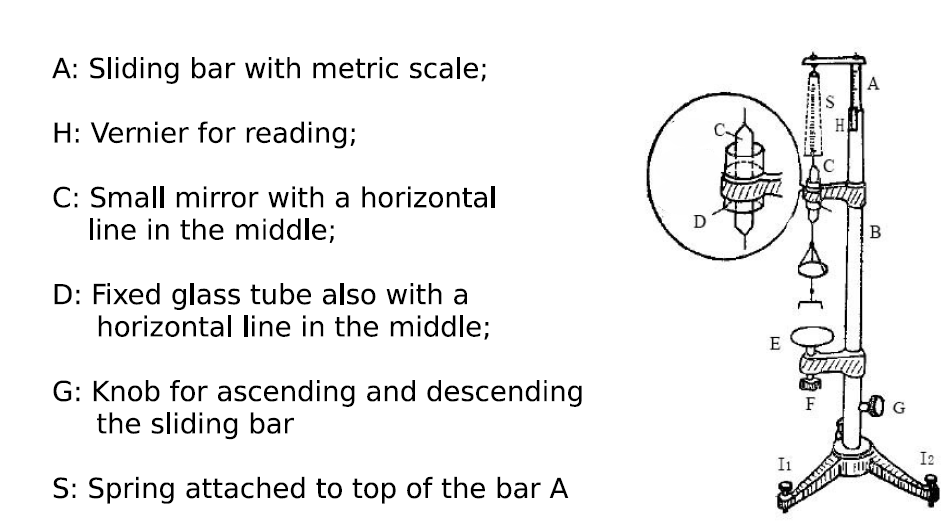
\includegraphics[scale=0.5]{P2.jpg}
\caption{Jolly balance}
\end{figure}
In order to measure the spring constant using the Jolly balance, we need to place the
small mirror $C$ in the tube $D$ and make three lines coincide: the line on  the mirror, the line on the glass tube and its reflection in the mirror. First, without
adding any weight on the bottom end of the spring, adjust the knob $G$ and make the
three lines coincide. Then read the scale $L_1$.
\par Second, add mass $m$ to the button of the spring. The spring is stretched and the three lines no longer coincide. Adjust knob $G$ to make them into one line again and read the corresponding number on scale $L_2$. The spring constant may be then found as
\begin{equation}
k=\frac{mg}{L_2-L_1}
\end{equation}
With a series of measurement for different masses $m$, we may estimate the spring constant by finding a linear fit to the data using the least squares method.
\begin{figure}[H]
\centering
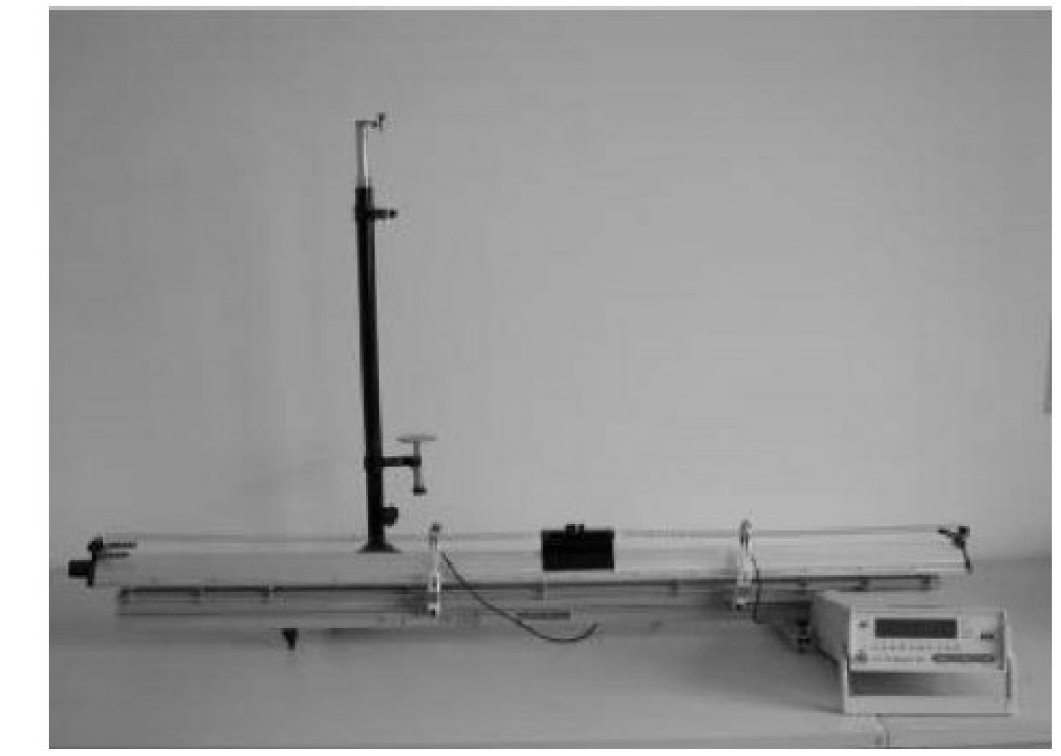
\includegraphics[scale=0.5]{P3.jpg}
\caption{The experiment setup.}
\end{figure}
\par A photoelectric measuring system consists of two photoelectric gates and an electronic timer. When a shutter placed on the object passes a gate, it blocks the light emitted from the light source at the top of the gate, and the receiver sends a signal to the electronic timer. Please note that for period measurements we use, we use the I-shape shutter.
\begin{figure}[H]
\centering
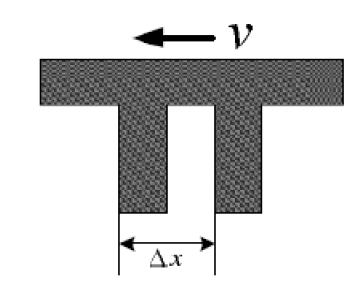
\includegraphics[scale=0.5]{P4.jpg}
\caption{The U-shape shutter.}
\end{figure}
When measuring the speed of the object, we use a U-shaped shutter (Figure 4), so
that the light is blocked twice during a pass. The timer will then record the time interval $\bigtriangleup t$ between the two generated signals. After the distance $\bigtriangleup x=\frac{1}{2}(x_{in}+x_{out})$ between the two arms of the U-shape shutter is measured, the speed of the object at the point of passing the gate is calculated as $v=\frac{\bigtriangleup x}{\bigtriangleup t}$.	
\section{Measurement Procedure}
\subsection{Spring Constant}
\begin{enumerate}
\item Adjust the Jolly balance to be vertical: Attach the spring and the mirror as shown
in Figure 2. Add a 20 g \textbf{preload} and adjust knob $I_1$ and $I_2$ to make sure the mirror
can move freely through the tube.\\ 
Check whether the Jolly balance is parallel to the spring, and adjust knobs if necessary. You should look at the balance from two orthogonal directions: from one direction, adjust the balance to be parallel to the spring; from the direction orthogonal to the previous one, check if the balance coincides with the spring.
\item Adjust knob $G$ and make the three lines in the tube coincide. Adjust the position of the tube to set the initial position $L_0$ within $5.0\sim10.0$ cm.
\item Record the reading $L_0$ on the scale, add mass $m_1$ and record $L_1$.
\item Keep adding masses and take measurements for six different positions. The order
of the masses should be recorded.
\item Estimate the spring constant $k_1$ using the least squares method.
\item Replace spring 1 with spring 2, repeat the measurements and calculate $k_2$.
\item Remove the preload and repeat the measurement for springs 1 and 2 connected in series. Calculate $k_3$ and compare it with the theoretical value.
\end{enumerate}
\subsection{Relation Between the Oscillation Period $T$ and the Mass of the Oscillator $M$}
\begin{enumerate}[(a)]
\item Adjust the air track so that it is horizontal.
\begin{enumerate}
\item Turn on the air pump and check if any of the holes on the air track are blocked.
Call the instructor for help if you find blocked holes.
\item Place the cart on the track without any initial velocity. Adjust the track until the object moves slowly back and forth in both directions.
\par \emph{Adjustment method.} The air track has three knobs at the bottom: two on one side
and another one on the other side. You can only adjust that single knob.
\end{enumerate}
\item Horizontal air track
\begin{enumerate}
\item Attach springs to the sides of the cart, and set up the I-shape shutter. Make sure
that the photoelectric gate is at the equilibrium position.
\item Add weight $m_1$. Let the cart oscillate about the photoelectric gate. The amplitude
of oscillations should be about 5 cm. Release the cart with a caliper or a ruler. Set
the timer into the "T" mode. The timer in this mode will automatically record
the time of 10 oscillation periods. Record the mass of the cart and the period.
\item Add weights to the object, repeat Step 2 and take measurements for 5 times.
\item Analyze the relation between $M$ and $T$ by plotting a graph.
\end{enumerate}
\item Inclined air track
\begin{enumerate}
\item Inclination of the air track is controlled with plastic plates. Place them under the
air track, using three plates at a time.
\item Repeat the steps in (b) for two different inclinations (for example, with 3 and 6 plates
beneath the air track).
\item Discuss the relation between $M$ and $T$ by plotting a graph.
\end{enumerate}
\end{enumerate}
\subsection{Relation Between the Oscillation Period $T$ and the Amplitude $A$}
\begin{enumerate}
\item Keep the mass of the cart unchanged and change the amplitude (choose 6 different
values). The recommended amplitude is about 5.0/ 10.0/ 15.0/ ... /30.0 cm.
\item Apply linear fit to the data and comment on the relation between the oscillation period
$T$ and the amplitude $A$ based on the correlation coefficient $\gamma$.
\end{enumerate}
\subsection{Relation Between the Maximum Speed and the Amplitude}
\begin{enumerate}
\item Measure the outer distance $x_{out}$ and the inner distance $x_{in}$ of the U-shape shutter by
a caliper. Calculate the distance $\bigtriangleup x=(x_{out} +x_{in})=2$.
\item Change the shutter from I- to U-shape. Set the timer into the "$S_1$" mode. Let the cart
oscillate. Record the second readings of the time interval $\bigtriangleup t$ only if the two subsequent readings show the same digits to the left of the decimal point.
\item Change the amplitude (choose 6 different values). The recommended amplitude is
about 5.0/ 10.0/ 15.0/ ... /30.0 cm.
\item Measure the maximum speed $v_max$ for different values of the amplitude $A$. Obtain the
spring constant from equation (6). Compare this result to that of the first part.
\end{enumerate}
\subsection{Mass measurement}
\begin{enumerate}
\item Adjust the electronic balance every time before you use it. The level bubble should be
in the center of the circle.
\item Add weights according to a fixed order. Weigh the cart with the I-shape shutter and
with the U-shape shutter. Measure the mass of spring 1 and spring 2.
\item Record the data only after the circular symbol on the scales display disappears.
\end{enumerate}
\section{Calculation and Results}
\subsection{Measurement Results}
\subsubsection{Spring Constant Measurement Data}
\begin{table}[H]
\centering
\begin{tabular}{|c|c|c|c|c|c|}
\hline
\multicolumn{2}{|c|}{spring 1 {[}mm{]} $\pm$ 0.1{[}mm{]}} & \multicolumn{2}{c|}{spring 2 {[}mm{]} $\pm$ 0.1{[}mm{]}} & \multicolumn{2}{c|}{spring 3 {[}mm{]} $\pm$ 0.1{[}mm{]}} \\ \hline
$L_0$                           & 105.0     &      $L_0$            & 65.5                 &    $L_0$              & 50.0                 \\ \hline
$L_1$                             & 125.0     &    $L_1$               & 84.6                 &   $L_1$                & 91.2                 \\ \hline
   $L_2$                           & 147.2     &      $L_2$             & 106.6                &    $L_2$               & 134.6                \\ \hline
    $L_3$                          & 168.5     &      $L_3$             & 126.3                &      $L_3$             & 178.0                \\ \hline
      $L_4$                        & 188.6     &       $L_4$           & 147.3                &       $L_4$           & 217.3                \\ \hline
     $L_5$                        & 210.0     &    $L_5$             & 168.5                &       $L_5$          & 260.5                \\ \hline
$L_6$     & 230.0     &      $L_6$             & 189.1                &   $L_6$   & 301.6                \\ \hline
\end{tabular}
\caption{Spring constant measurement data}
\end{table}
\subsubsection{Time Measurements of Ten Periods for T vs. M Relation}
\begin{table}[H]
\centering
\begin{tabular}{|c|c|c|c|c|c|}
\hline
\multicolumn{6}{|c|}{Ten periods {[}ms{]} $\pm$ 0.1{[}ms{]}}                                           \\ \hline
\multicolumn{2}{|c|}{horizontal} & \multicolumn{2}{c|}{incline 1} & \multicolumn{2}{c|}{incline 2} \\ \hline
$m_1$            & 12893.6           &  $m_1$          & 12897.1           &           $m_1$ & 12897.0           \\ \hline
$m_2$             & 13059.8           &  $m_2$              & 13058.5           &           $m_2$     & 13057.2           \\ \hline
$m_3$                 & 13213.2           &    $m_3$         & 13215.0           &           $m_3$  & 13215.0           \\ \hline
$m_4$              & 13373.7           &   $m_4$         & 13371.5           &            $m_4$& 13371.5           \\ \hline
$m_5$             & 13529.2           &   $m_5$         & 13528.1           &           $m_5$ & 13526.0           \\ \hline
$m_6$         & 13682.2           &    $m_6$        & 13680.2           &     $m_6$       & 13677.3           \\ \hline
\end{tabular}
\caption{Data for the T vs. M relation}
\end{table}
\subsubsection{Time Measurements of Ten Periods for T vs. A Relation}
\begin{table}[H]
\centering
\begin{tabular}{|c|c|c|}
\hline
\multicolumn{2}{|c|}{A {[}mm{]} $\pm$ 1{[}mm{]}} & ten periods {[}ms{]} $\pm$ 0.1{[}ms{]} \\ \hline
1                   & 50                   & 12731.3                          \\ \hline
2                   & 100                  & 12734.1                          \\ \hline
3                   & 150                  & 12736.2                          \\ \hline
4                   & 200                  & 12735.3                          \\ \hline
5                   & 250                  & 12734.1                          \\ \hline
6                   & 300                  & 12733.7                          \\ \hline
\end{tabular}
\caption{Data for the T vs. A relation}
\end{table}
\subsubsection{Measurement Data for the $v_{max}^2$ vs. $A^2$ Relation}
\begin{table}[H]
\centering
\begin{tabular}{|c|c|c|}
\hline
\multicolumn{2}{|c|}{$A$ {[}mm{]} $\pm$ 1{[}mm{]}}    & $\bigtriangleup{t}$ {[}ms{]} $\pm$ 0.1{[}ms{]}   \\ \hline
1                     & 50                     & 40.55                    \\ \hline
2                     & 100                    & 20.49                    \\ \hline
3                     & 150                    & 13.84                    \\ \hline
4                     & 200                    & 10.35                    \\ \hline
5                     & 250                    & 8.24                     \\ \hline
6                     & 300                    & 6.89                     \\ \hline
\multicolumn{2}{|c|}{$x_{in}$ {[}mm{]} $\pm$ 0.02{[}mm{]}} & $x_{out}$ {[}mm{]} $\pm$ 0.02{[}mm{]} \\ \hline
\multicolumn{2}{|c|}{4.20}                     & 15.44                    \\ \hline
\multicolumn{2}{|c|}{4.12}                     & 15.24                    \\ \hline
\multicolumn{2}{|c|}{4.14}                     & 15.56                    \\ \hline
\end{tabular}
\caption{Data for the $v_{max}^2$ vs. $A^2$ relation}
\end{table}
\subsubsection{Measurement Data for Weight}
\begin{table}[H]
\centering
\begin{tabular}{|c|c|}
\hline
\multicolumn{2}{|c|}{m{[}g{]} $\pm$ 0.01{[}g{]}} \\ \hline
1                  & 4.66                  \\ \hline
2                  & 9.47                  \\ \hline
3                  & 14.12                 \\ \hline
4                  & 18.88                 \\ \hline
5                  & 23.67                 \\ \hline
6                  & 28.42                 \\ \hline
\end{tabular}
\caption{Weight measurement data}
\end{table}
\subsubsection{Mass Measurement Data}
\begin{table}[H]
\centering
\begin{tabular}{|c|}
\hline
object with I-shape $m_{obj}${[}g{]} $\pm$ 0.01{[}g{]} \\ \hline
178.08                                   \\ \hline
object with U-shape $m_{obj}${[}g{]} $\pm$ 0.01{[}g{]} \\ \hline
187.19                                   \\ \hline
mass of spring 1 $m_{spr1}${[}g{]} $\pm$ 0.01{[}g{]}    \\ \hline
11.23                                    \\ \hline
mass of spring 2 $m_{spr2}${[}g{]} $\pm$ 0.01{[}g{]}    \\ \hline
10.72                                    \\ \hline
\end{tabular}
\caption{Mass measurement data}
\end{table}
\subsubsection{Other Relative Data}
\begin{table}[H]
\centering
\begin{tabular}{|c|}
\hline
g {[}m/s{]}             \\ \hline
9.794                   \\ \hline
mass of preload {[}g{]} \\ \hline
20                      \\ \hline
\end{tabular}
\caption{Acceleration due to gravity and mass of preload}
\end{table}
\subsection{Calculations}
\subsubsection{Calculation of Equivalent Mass $M_0$}
$$M_0=m_{obj}+\frac{1}{3}m_{spr1}+\frac{1}{3}m_{spr2}$$
$$M_I=178.08+\frac{1}{3}\times11.23+\frac{1}{3}\times10.72=185.40[g]$$
$$M_U=187.19+\frac{1}{3}\times11.23+\frac{1}{3}\times10.72=194.51[g]$$
\subsubsection{Calculation of $\bigtriangleup{x}$, $v$, and $mv^2$}
$$\bar{x}_{in}=\frac{1}{3}(4.20+4.12+4.14)=4.15[mm]$$
$$\bar{x}_{out}=\frac{1}{3}(15.44+15.24+15.56)=15.41[mm]$$
$$\bigtriangleup{x}=\frac{1}{2}(\bar{x}_{in}+\bar{x}_{out})=\frac{1}{2}(4.15+15.41)=9.78[mm]$$
$$v=\frac{\bigtriangleup{x}}{\bigtriangleup{t}}$$
$$v_1=\frac{\bigtriangleup{x}}{\bigtriangleup{t}_1}=\frac{9.78}{40.55}=0.24[m/s]$$
$$m{v_1}^2=194.51\times(0.24)^2=1.1\times{10^{-2}}[kg\cdot{m^2}/{s^2}]$$
\begin{table}[H]
\centering
\begin{tabular}{|c|c|c|c|}
\hline
  & $\bigtriangleup{t}$ {[}ms{]} $\pm$ 0.1{[}ms{]}& $v$[m/s]&$mv^2[kg\cdot{m^2}/{s^2}]$  \\ \hline
1 & 40.55 & 0.24 & $1.1\times{10^{-2}}$ \\ \hline
2 & 20.49 & 0.48 &$4.5\times{10^{-2}}$\\ \hline
3 & 13.84 & 0.71 &$9.8\times{10^{-2}}$\\ \hline
4 & 10.35 & 0.94 &$1.7\times{10^{-1}}$\\ \hline
5 & 8.24  & 1.19 &$2.8\times{10^{-1}}$\\ \hline
6 & 6.89  & 1.42 &$3.9\times{10^{-1}}$\\ \hline
\end{tabular}
\caption{Calculated data for $v_{max}$ and $mv^2$}
\end{table}
\subsection{Theoretical Value k from data measured by Jolly balance}
At the first of the measurement procedure, I used a Jolly balance to measure the spring constant of $k_1$, $k_2$, and $k_1+k_2$ indirectly. The Jolly balance can recorded the length of spring when its restoring force is increasing, then I can get its k through linear fit diagram. The restoring force equals to the total weight connected to the spring
$$F_1=(m_p+m_1)g=(20+4.66)\times9.794=241.52[mN]$$
\begin{table}[H]
\centering
\begin{tabular}{|c|c|c|c|c|c|c|c|}
\hline
\multicolumn{2}{|c|}{spring 1 {[}mm{]} $\pm$ 0.1{[}mm{]}} & \multicolumn{2}{c|}{spring 2 {[}mm{]} $\pm$ 0.1{[}mm{]}} & \multicolumn{2}{c|}{spring 3 {[}mm{]} $\pm$ 0.1{[}mm{]}}& \multicolumn{2}{c|}{mg[mN] $\pm$ 0.1[mN]} \\ \hline
$L_0$                           & 105.0     &      $L_0$            & 65.5                 &    $L_0$              & 50.0 &$F_0$     &195.88           \\ \hline
$L_1$                             & 125.0     &    $L_1$               & 84.6                 &   $L_1$                & 91.2  &$F_1$   &241.52            \\ \hline
   $L_2$                           & 147.2     &      $L_2$             & 106.6                &    $L_2$               & 134.6 &$F_2$   &288.63            \\ \hline
    $L_3$                          & 168.5     &      $L_3$             & 126.3                &      $L_3$             & 178.0 &$F_3$   &334.17           \\ \hline
      $L_4$                        & 188.6     &       $L_4$           & 147.3                &       $L_4$           & 217.3  &$F_4$   &380.79           \\ \hline
     $L_5$                        & 210.0     &    $L_5$             & 168.5                &       $L_5$          & 260.5  &$F_5$    &427.70          \\ \hline
$L_6$     & 230.0     &      $F_6$             & 189.1                &   $L_6$   & 301.6   &$F_6$      &474.23       \\ \hline
\end{tabular}
\caption{Indirect spring constant measurement data}
\end{table}
\begin{figure}[H]
\centering
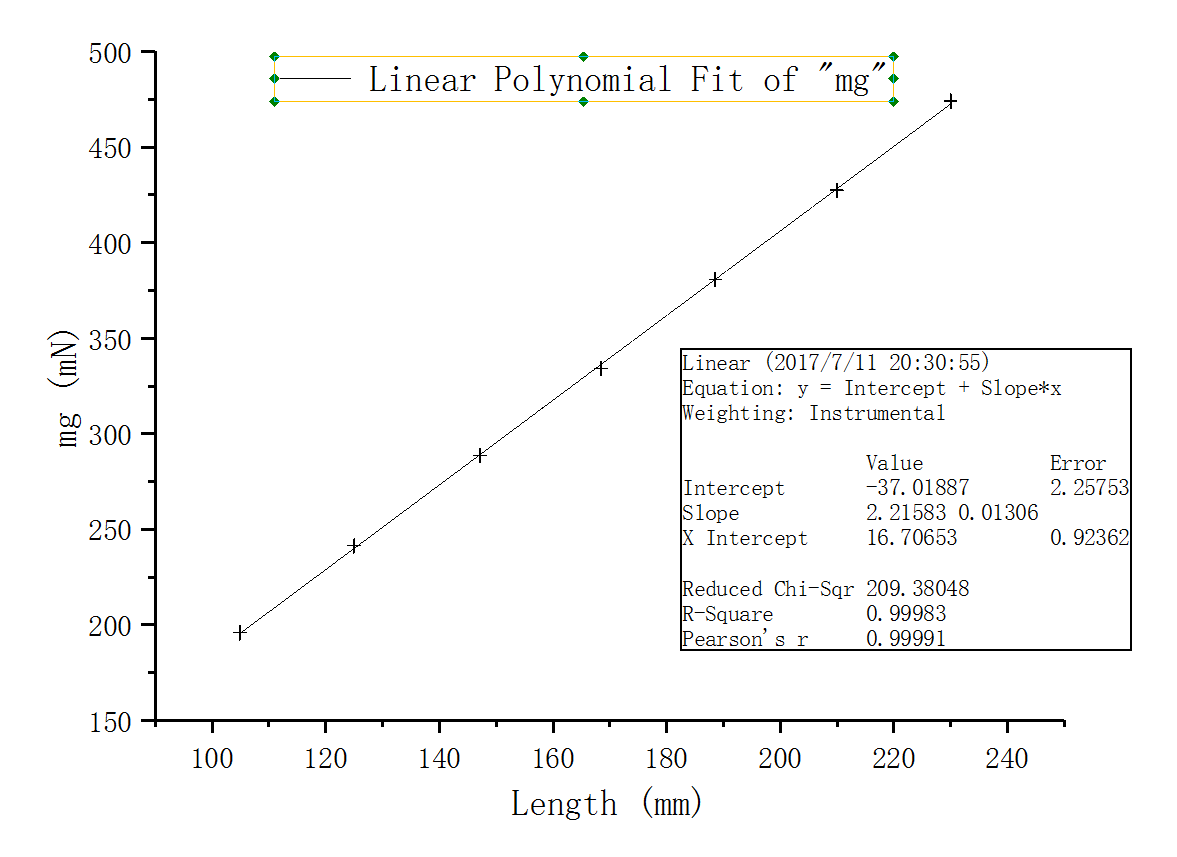
\includegraphics[scale=0.4]{P5.jpg}
\caption{The linear fit diagram for spring 1.}
\end{figure}
Through the linear fir diagram, I know $k_{spr1}=2.216\pm0.013$[N/m] 
\begin{figure}[H]
\centering
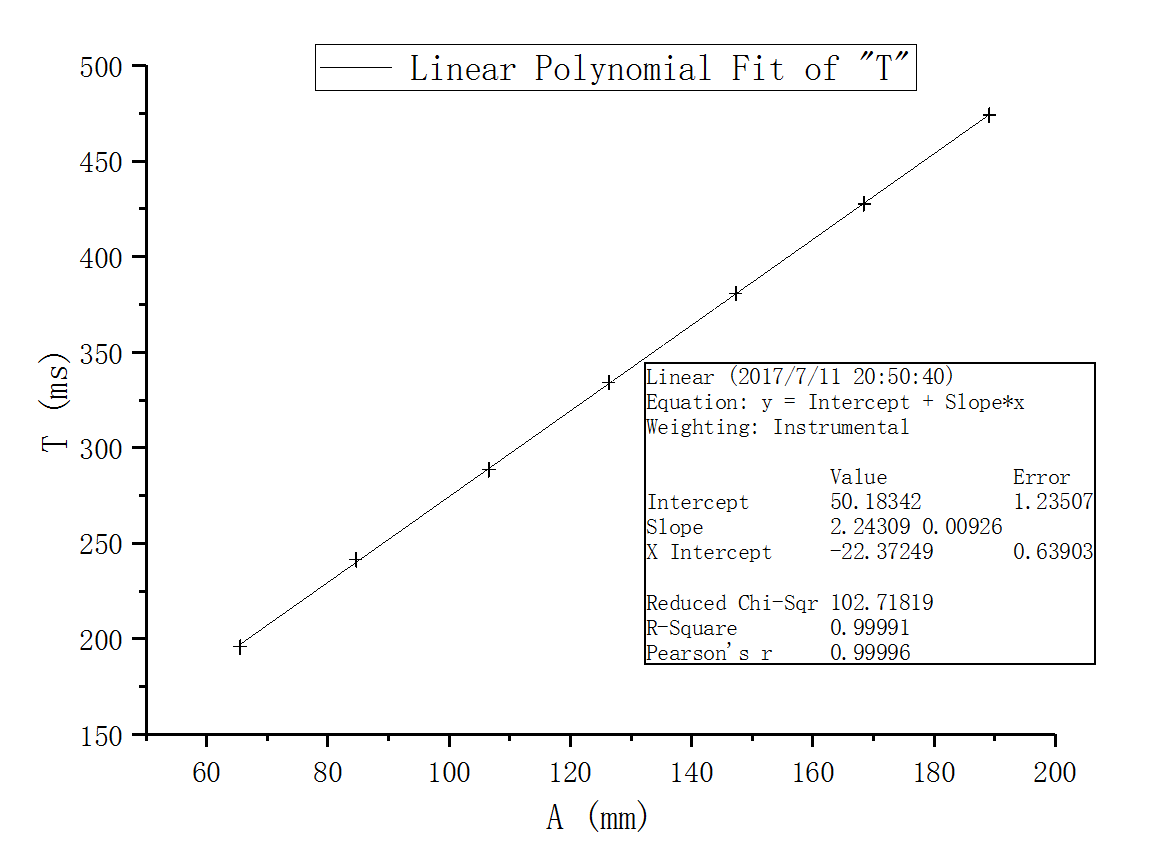
\includegraphics[scale=0.4]{P6.jpg}
\caption{The linear fit diagram for spring 2.}
\end{figure}
Through the linear fir diagram, I know $k_{spr2}=2.243\pm0.009$[N/m] 
When I measured the k of the series, I didn't use preload, but the result should be same because k is only relative the change of F, so I can use the data for measurement of $k_{spr1}$ and $k_{spr2}$.
\begin{figure}[H]
\centering
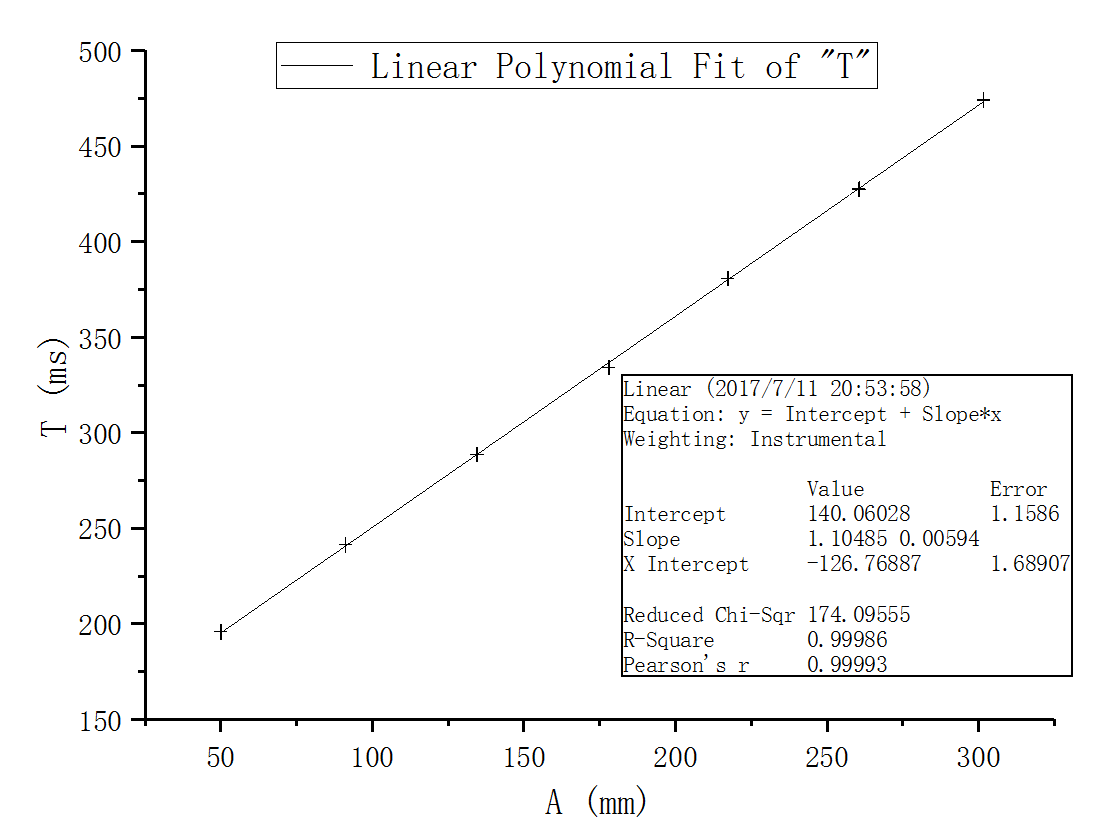
\includegraphics[scale=0.4]{P7.jpg}
\caption{The linear fit diagram for series.}
\end{figure}
Through the linear fit diagram, I know $k_{sp1+sp2}=1.105\pm0.006$[N/m] 
\subsection{Diagram for Relation between T and M}
Preload was no longer used after the measurement of spring constant, so M is equal to the weight measurement data but I have to add the equivalent mass of object with I-shape. 
$$m_1=4.66+185.40=190.06[g]=0.19[kg]$$
In addition, since T is proportional to $\sqrt{M}$, I use square of one period $T^2$ as y coordinates to draw the linear fit graph.
\begin{table}[H]
\centering
\begin{tabular}{|c|c|c|c|c|c|c|}
\hline
\multicolumn{6}{|c|}{Periods {[}s$^2${]}}    &M[kg] $\pm2\times10^{-5}[kg]$ \\ \hline
\multicolumn{2}{|c|}{horizontal} & \multicolumn{2}{c|}{incline 1} & \multicolumn{2}{c|}{incline 2}& \\ \hline
$m_1$            & 1.6624           &  $m_1$          & 1.6634           &           $m_1$ & 1.6633 &0.1901         \\ \hline
$m_2$             & 1.7056           &  $m_2$              & 1.7052           &           $m_2$     & 1.7049  &0.1949         \\ \hline
$m_3$                 & 1.7459           &    $m_3$         & 1.7464           &           $m_3$  & 1.7464  &0.1995          \\ \hline
$m_4$              & 1.7886           &   $m_4$         & 1.7880           &            $m_4$& 1.7880     &0.2042       \\ \hline
$m_5$             & 1.8304           &   $m_5$         & 1.8301           &           $m_5$ & 1.8295    &0.2091        \\ \hline
$m_6$         & 1.8720           &    $m_6$        & 1.8715           &     $m_6$       & 1.8707 &0.2138           \\ \hline
\end{tabular}
\caption{Data for the T vs. M relation}
\end{table}
\begin{figure}[H]
\centering
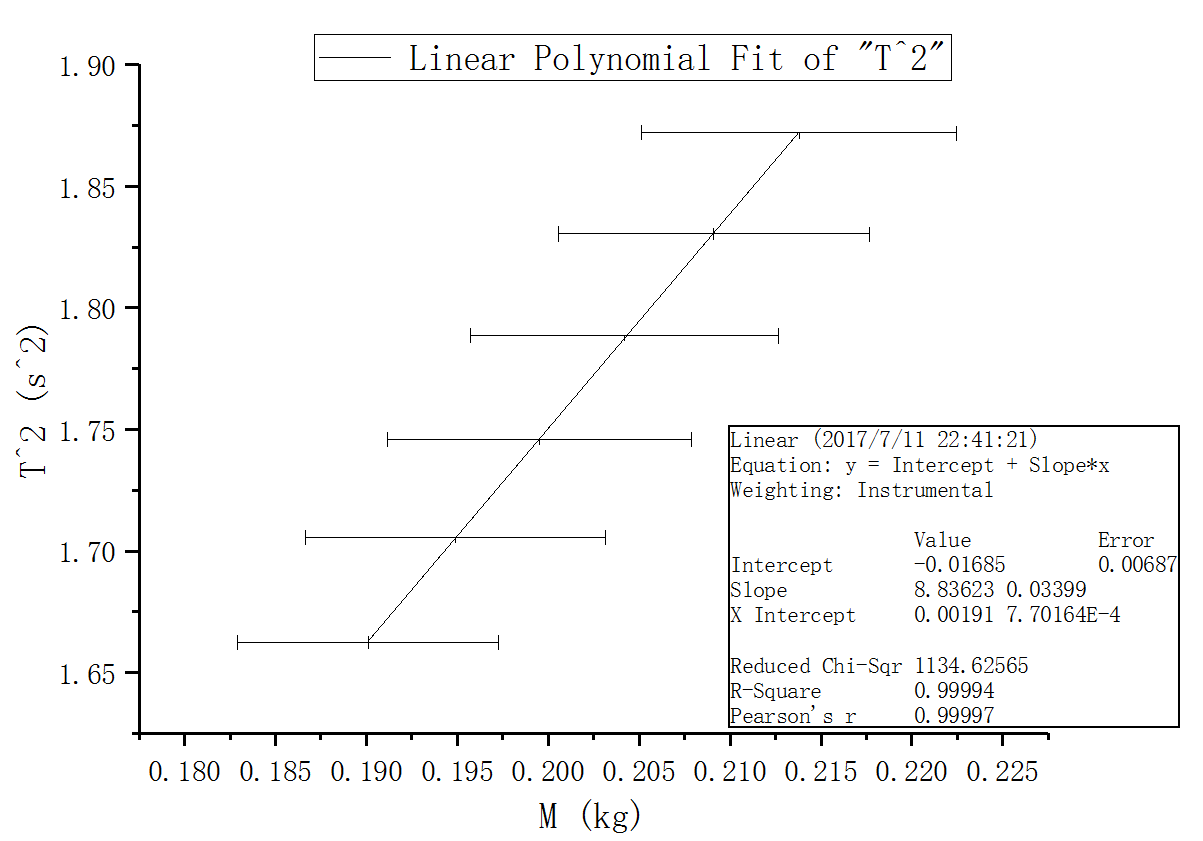
\includegraphics[scale=0.4]{P8.jpg}
\caption{The linear fit diagram for $T^2$ vs. M when air track is horizontal.}
\end{figure}
From the diagram, I can see that $T^2$ is proportional to the value of M when the air track is horizontal. Then I will examine what will happen when the track form an incline with the ground. (The uncertain of error bar is in the uncertainty analysis section)
\begin{figure}[H]
\centering
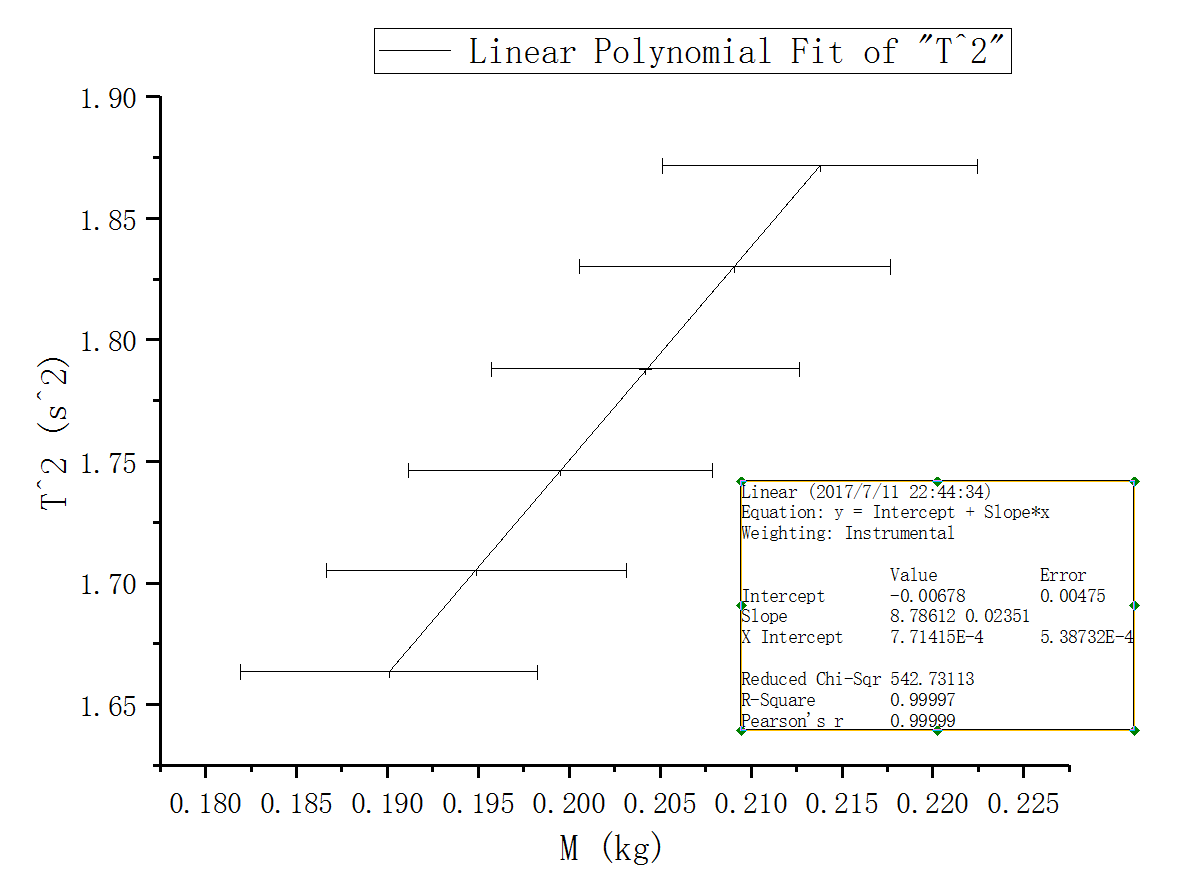
\includegraphics[scale=0.4]{P9.jpg}
\caption{The linear fit diagram for $T^2$ vs. M when air track forms an incline 1.}
\end{figure}
\begin{figure}[H]
\centering
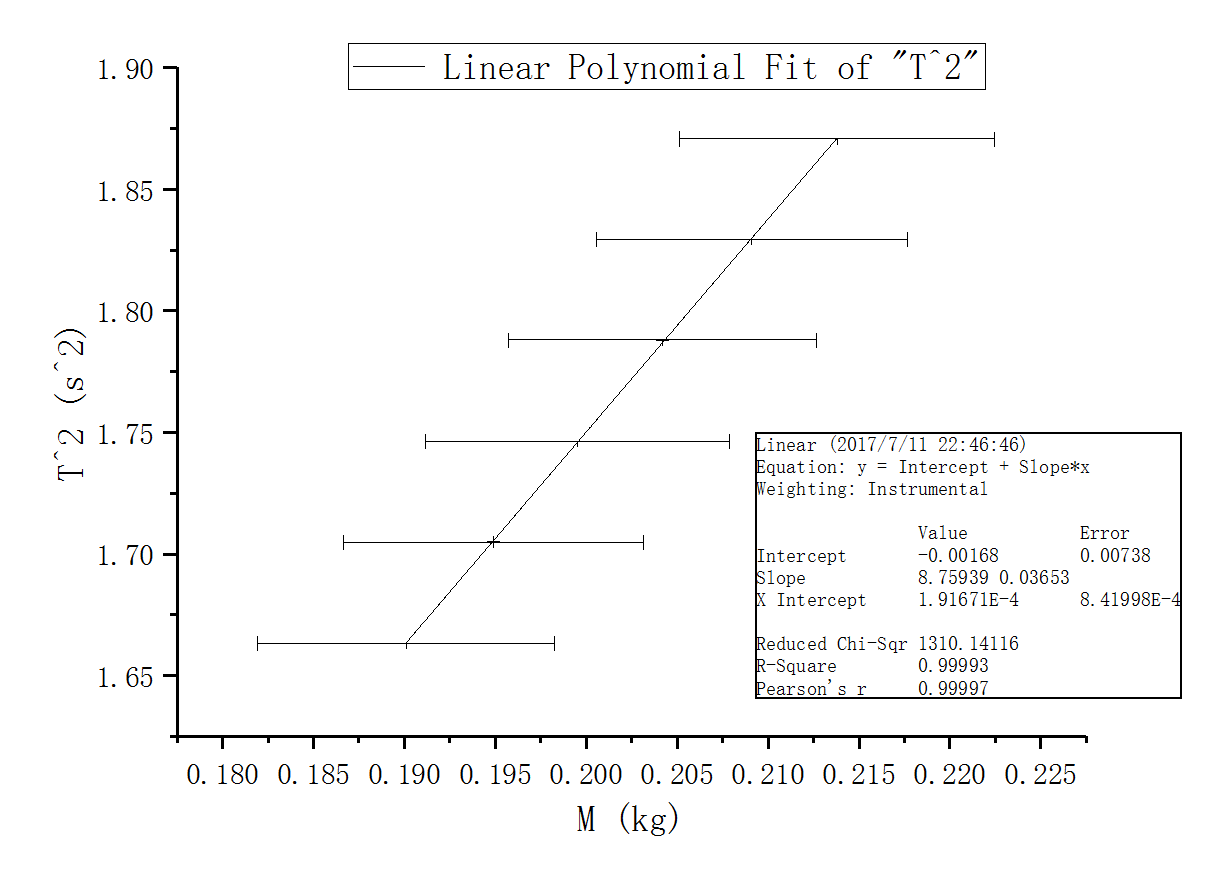
\includegraphics[scale=0.4]{P10.jpg}
\caption{The linear fit diagram for $T^2$ vs. M when air track forms an incline 2.}
\end{figure}
From the three diagrams we can see the three slope is $k_1=8.836\pm0.034$, $k_2=8.786\pm0.024$, and $k_3=8.759\pm0.037$, which are very close. As a result, I think the angle between the air track and ground has no effect on the relation between T and M.
\subsection{Diagram for Relation between T and A}
\begin{table}[H]
\centering
\begin{tabular}{|c|c|c|}
\hline
  & A[mm]$\pm$1[mm] & ten periods [ms] $\pm$ 0.1[ms]\\ \hline
1 & 50    & 12731.3   \\ \hline
2 & 100      & 12734.1   \\ \hline
3 & 150     & 12736.2   \\ \hline
4 & 200      & 12735.3   \\ \hline
5 & 250     & 12734.1 \\ \hline
6 & 300      & 12733.7   \\ \hline
\end{tabular}
\caption{Data for $T$ vs. $A$ relation}
\end{table}
\begin{figure}[H]
\centering
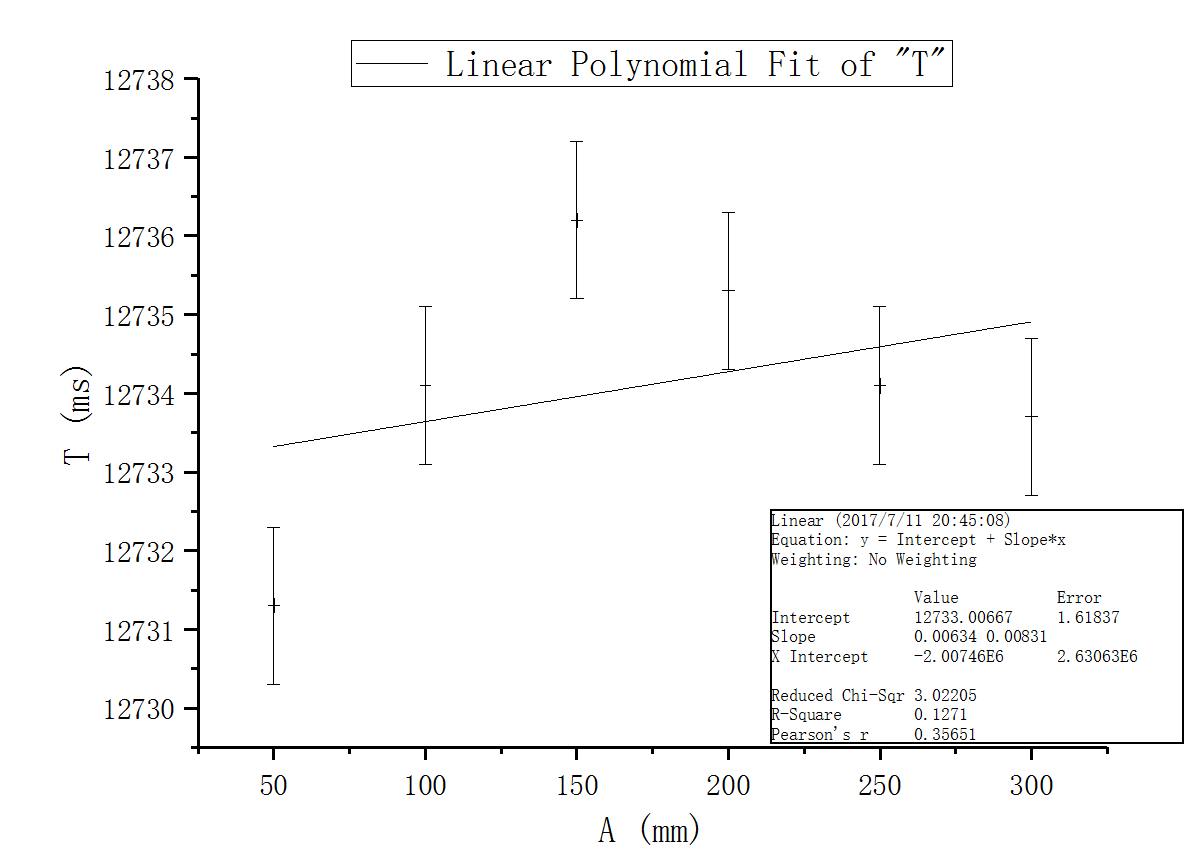
\includegraphics[scale=0.4]{P11.jpg}
\caption{The linear fit diagram for $T$ vs. A relation.}
\end{figure}
From the diagram I can see that the slope is very small but it still fit all the points. It seems that all the points on the diagram is not well distributed so A has nothing to do with T.
\subsection{Diagram for Relation between $v_{max}^2$ vs. $A^2$} 
\begin{table}[H]
\centering
\begin{tabular}{|c|c|c|}
\hline
  & A$^2$[m$^2$] & $v_{max}^2[m^2/s^2]$ \\ \hline
1 & 0.0025    & 0.0576   \\ \hline
2 & 0.0100      & 0.2304   \\ \hline
3 & 0.0225     & 0.5041   \\ \hline
4 & 0.0400      & 0.8836   \\ \hline
5 & 0.0625     & 1.4161   \\ \hline
6 & 0.0900      & 2.0164   \\ \hline
\end{tabular}
\caption{Data for $v_{max}^2$ vs. $A^2$ relation}
\end{table}
\begin{figure}[H]
\centering
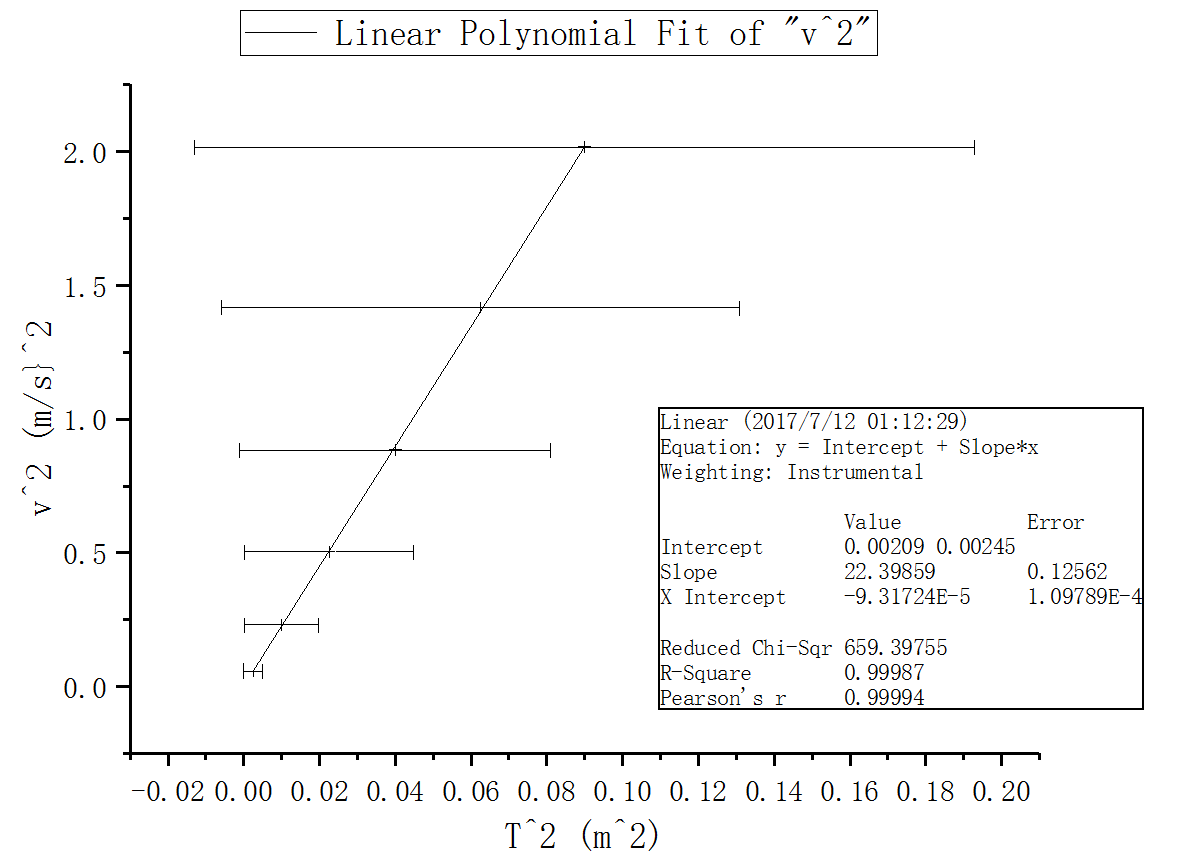
\includegraphics[scale=0.4]{P12.jpg}
\caption{The linear fit diagram for  $v_{max}^2$ vs. $A^2$.}
\end{figure}
From the diagram I know that the slope between $v_{max}^2$ and $A^2$ is 22.42 $\pm$ 0.14 [1/$s^2$], so V is proportional to A. According to equation (6), $k=M_U\times{slope}=0.194\times22.42=4.36\pm0.027[N/m]$
\section{Measurement Uncertainty Analysis}
\subsection{Multiple Measurements Yield to Type A Uncertainty}
For multiple measurements' uncertainty:
$$\bar{X}=\frac{1}{n}\sum_{i=1}^nx_i$$
$$S_X=\sqrt{\frac{1}{n-1}\sum_{i=1}^n(x_i-\bar{X})^2}$$  
$$\bigtriangleup_A=\frac{S_Xt_{0.95}}{\sqrt{n}}$$
The value of $t_{0.95}$ and $\frac{t_{0.95}}{\sqrt{n}}$ are giving in Table 7 
\begin{table}[H]
\centering
\begin{tabular}{|l|l|l|l|l|l|l|l|l|l|l|l|}
\hline
n                         & 3    & 4    & 5     & 6    & 7     & 8     & 9     & 10    & 15    & 20    & $\ge100$   \\ \hline
$t_{0.95}$                  & 4.30 & 3.18 & 2.78  & 2.57 & 2.45  & 2.36  & 2.31  & 2.26  & 2.14  & 2.09  & $\le1.97$  \\ \hline
$\frac{t_0.95}{\sqrt{n}}$ & 2.48 & 1.59 & 1.204 & 1.05 & 0.926 & 0.834 & 0.770 & 0.715 & 0.553 & 0.467 & $\le0.139$ \\ \hline
\end{tabular}
\caption{The values of $t_{0.95}$ and $\frac{t_{0.95}}{\sqrt{n}}$}
\end{table}
\subsubsection{Type A Uncertainty for $x_{in}$ and $x_{out}$ }
$$\bar{x}_{in}=\frac{1}{3}(4.20+4.12+4.14)=4.15[mm]$$
$$S_x=\sqrt{\frac{1}{2}\sum_{i=1}^3(x_i-\bar{x}_{in})^2}=0.04$$
$$\bigtriangleup_A=\frac{S_Xt_{0.95}}{\sqrt{n}}=0.04\times\frac{4.3}{\sqrt{3}}=0.099[mm]$$
$$\bar{x}_{out}=\frac{1}{3}(15.44+15.24+15.56)=15.41[mm]$$
$$S_x=\sqrt{\frac{1}{2}\sum_{i=1}^3(x_i-\bar{x}_{out})^2}=0.16$$
$$\bigtriangleup_A=\frac{S_Xt_{0.95}}{\sqrt{n}}=0.16\times\frac{4.3}{\sqrt{3}}=0.397[mm]$$
\subsection{Uncertainty for $x_{in}$, $x_{out}$, and $\bigtriangleup{x}$}
Since $\bigtriangleup_B=0.02[mm]$ then
$$u_{in}=\sqrt{\bigtriangleup_A^2+\bigtriangleup_B^2}=\sqrt{0.02^2+0.172^2}=0.101[mm]$$
$$u_r=\frac{u_{in}}{\bar{x}_{in}}\times100\%=\frac{0.101}{4.15}\times100\%=2.43\%$$
Similarly, $u_{out}=0.398[mm]$ and $u_r=2.58\%$
$$\bigtriangleup{x}=\frac{1}{2}(x_{in}+x_{out})$$
$$u_{\bigtriangleup{x}}=\sqrt{(\frac{\partial{\bigtriangleup{x}}}{\partial{x_{in}}}\cdot{u_{in}})^2+(\frac{\partial{\bigtriangleup{x}}}{\partial{x_{in}}}\cdot{u_{out}})^2}=\sqrt{(\frac{0.101}{2})^2+(\frac{0.398}{2})^2}=0.205[mm]$$
$$u_r=\frac{u_{\bigtriangleup{x}}}{\bigtriangleup{x}}\times100\%=\frac{0.716}{9.78}\times100\%=2.10\%$$
\begin{table}[H]
\centering
\begin{tabular}{|c|c|c|c|}
\hline
  & Value {[}m{]} & Uncertainty {[}m{]} & Relative uncertainty \% \\ \hline
$x_{in}$ & 4.15$\times10^{-3}$          &       1.01$\times10^{-4}$              & 2.43\%                  \\ \hline
$x_{out}$ & 1.541$\times10^{-2}$          &          3.98$\times10^{-4}$           & 2.58\%                  \\ \hline
$\bigtriangleup{x}$ & 9.78$\times10^{-3}$          &     2.05$\times10^{-4}$                 & 2.1\%                  \\ \hline
\end{tabular}
\caption{Uncertainty for $x_{in}$, $x_{out}$, and $\bigtriangleup{x}$}
\end{table}
\subsection{Uncertainty for Equivalent Mass}
$$u_M=m_{obj}+\frac{1}{3}m_{spr1}+\frac{1}{3}m_{spr}u_m=\sqrt{(\frac{\partial{M_0}}{\partial{m_{obj}}}\cdot{u_{m(obj)})^2}+(\frac{\partial{M_0}}{\partial{m_{spr1}}}\cdot{u_{m(spr1)})^2}+(\frac{\partial{M_0}}{\partial{m_{spr2}}}\cdot{u_{m(spr2)})^2}}$$
$$u_I=u_U=\sqrt{0.01^2+(\frac{1}{3}\times0.01)^2+(\frac{1}{3}\times0.01)^2}=1\times10^{-5}[kg]$$
$$u_{rI}=\frac{u_I}{M_I}\times100\%=\frac{0.011}{185.4}\times100\%=0.01\%$$
$$u_{rU}=\frac{0.011}{194.51}\times100\%=0.01\%$$
\subsection{Uncertainty for T vs. M Relation}
Since I draw a picture of $T^2$ and M, I must calculate the uncertainty of $T^2$ and M.
$$T^2=(\frac{t}{10})^2$$
$$u_{T^2}=\sqrt{(\frac{\partial{T^2}}{\partial{t}}\cdot{u_t})^2}=\sqrt{\frac{2t}{5}\times10^{-4}}$$
$$u_1=\sqrt{0.4\times10^{-4}\times1.28936}=7.18\times10^{-3}[s^2]$$
$$u_r=\frac{u_1}{T^2}\times100\%=\frac{7.18\times10^{-3}}{1.6624}\times100\%=0.43\%$$
\begin{table}[H]
\centering
\begin{tabular}{|c|c|c|c|}
\hline
\multicolumn{4}{|c|}{Horizontal}                \\ \hline
  & $T^2[s^2]$      & Uncertainty $[s^2]$ & Relative Uncertainty \% \\ \hline
$m_1$ & 1.6624 		  & $7.18\times10^{-3}$        & 0.43\%                \\ \hline
$m_2$  & 1.7056       & $8.26\times10^{-3}$            &   0.48\%                \\ \hline
$m_3$  & 1.7459       & $8.36\times10^{-3}$            &  0.48\%                    \\ \hline
$m_4$  & 1.7886       & $8.46\times10^{-3}$            &  0.47\%                    \\ \hline
$m_5$  & 1.8304       & $8.56\times10^{-3}$            &  0.47\%                    \\ \hline
$m_6$  & 1.8720       & $8.65\times10^{-3}$            &  0.46\%                      \\ \hline
\end{tabular}
\caption{Uncertainty for $T^2$ when air track is horizontal}
\end{table}
\begin{table}[H]
\centering
\begin{tabular}{|c|c|c|c|}
\hline
\multicolumn{4}{|c|}{Incline 1}                \\ \hline
  & $T^2[s^2]$      & Uncertainty $[s^2]$ & Relative Uncertainty \% \\ \hline
$m_1$ & 1.6634 		  & $8.16\times10^{-3}$        & 0.49\%                \\ \hline
$m_2$  & 1.7052       & $8.26\times10^{-3}$            &   0.48\%                \\ \hline
$m_3$  & 1.7464       & $8.36\times10^{-3}$            &  0.48\%                    \\ \hline
$m_4$  & 1.7880       & $8.46\times10^{-3}$            &  0.47\%                    \\ \hline
$m_5$  & 1.8301       & $8.56\times10^{-3}$            &  0.47\%                    \\ \hline
$m_6$  & 1.8715       & $8.65\times10^{-3}$            &  0.46\%                      \\ \hline
\end{tabular}
\caption{Uncertainty for $T^2$ when air track forms incline 1}
\end{table}
\begin{table}[H]
\centering
\begin{tabular}{|c|c|c|c|}
\hline
\multicolumn{4}{|c|}{Incline 2}                \\ \hline
  & $T^2[s^2]$      & Uncertainty $[s^2]$ & Relative Uncertainty \% \\ \hline
$m_1$ & 1.6633 		  & $8.16\times10^{-3}$        & 0.49\%                \\ \hline
$m_2$  & 1.7049       & $8.26\times10^{-3}$            &   0.48\%                \\ \hline
$m_3$  & 1.7464       & $8.36\times10^{-3}$            &  0.48\%                    \\ \hline
$m_4$  & 1.7880       & $8.46\times10^{-3}$            &  0.47\%                    \\ \hline
$m_5$  & 1.8295       & $8.55\times10^{-3}$            &  0.47\%                    \\ \hline
$m_6$  & 1.8707       & $8.65\times10^{-3}$            &  0.46\%                      \\ \hline
\end{tabular}
\caption{Uncertainty for $T^2$ when air track forms incline 2}
\end{table}
\subsection{Uncertainty for $A^2$ and $v^2$}
$$u_{A^2}=\sqrt{(2A\cdot{u_A})^2}$$
$$u_1=\sqrt{(2A_1)^2}=100[mm^2]=1\times{10^{-4}}[m^2]$$
$$u_r=\frac{u_1}{A_1^2}\times100\%=\frac{100}{2500}\times100\%=4\%$$
\begin{table}[H]
\centering
\begin{tabular}{|c|c|c|c|}
\hline
  & $A^2$ [$m^2$]   & Uncertainty [$m^2$] & Relative uncertainty \% \\ \hline
1 & 0.0025 & 1$\times10^{-4}$              & 4\%                     \\ \hline
2 & 0.0100     & 2$\times10^{-4}$        &   2\%                      \\ \hline
3 & 0.0225     & 3$\times10^{-4}$                 &  1.33\%                       \\ \hline
4 & 0.0400     & 4$\times10^{-4}$                 &    1\%                     \\ \hline
5 & 0.0625     & 5$\times10^{-4}$                 &    0.8\%                     \\ \hline
6 & 0.0900     & 6$\times10^{-4}$                 &    0.67\%                     \\ \hline
\end{tabular}
\caption{Uncertainty for $A^2$}
\end{table}
$$u_v=\sqrt{(\frac{\partial{v}}{\partial{\bigtriangleup{t}}}\cdot{u_{\bigtriangleup{t}}})^2+(\frac{\partial{v}}{\partial{\bigtriangleup{x}}}\cdot{u_{\bigtriangleup{x}}})^2}=\sqrt{(-\frac{\bigtriangleup{x}}{{\bigtriangleup{t}}^2}\cdot{u_{\bigtriangleup{t}}})^2+(\frac{1}{\bigtriangleup{t}}\cdot{u_{\bigtriangleup{x}}})^2}$$
$$u_{v1}=\sqrt{(-\frac{9.78\times10^{-3}}{{(4.06\times{10^{-2}}})^2}\cdot{10^{-4}})^2+(\frac{1}{4.06\times{10^{-2}}}\cdot{2.05\times10^{-4}})^2}=5.09\times{10^{-3}}[m/s]$$
$$u_{r1}=\frac{u_{v1}}{v_1}\times{100\%}=\frac{5.09\times{10^{-2}}}{0.24}=2.12\%$$
$$u_{v^2}=\sqrt{(\frac{\partial{v^2}}{\partial{v}}\cdot{u_v})^2}=2v\cdot{u_v}$$
$$u_{v_1^2}=2\times0.24\times5.09\times10^{-3}=2.44\times10^{-3}[m/s^2]$$
$$u_{r1}=\frac{u_{v_1^2}}{v_1^2}\times100\%=\frac{2.44\times10^{-3}}{0.0576}\times100\%=4.24\%$$
\begin{table}[H]
\centering
\begin{tabular}{|c|c|c|c|}
\hline
  & $v$ [$m/s$]   & Uncertainty [$m/s$] & Relative uncertainty \% \\ \hline
1 & 0.24 & 5.09$\times10^{-3}$              & 2.12\%                     \\ \hline
2 & 0.48     &1.02$\times10^{-2}$        &   2.13\%                      \\ \hline
3 & 0.71     & 1.57$\times10^{-2}$                 &  2.21\%                       \\ \hline
4 & 0.94     & 2.18$\times10^{-2}$                 &    2.32\%                     \\ \hline
5 & 1.19     & 2.87$\times10^{-2}$                 &    2.41\%                     \\ \hline
6 & 1.42     & 3.62$\times10^{-2}$                 &    2.55\%                     \\ \hline
\end{tabular}
\caption{Uncertainty for $v$}
\end{table}
\begin{table}[H]
\centering
\begin{tabular}{|c|c|c|c|}
\hline
  & $v^2$ [$(m/s)^2$]   & Uncertainty [$(m/s)^2$] & Relative uncertainty \% \\ \hline
1 & 0.0576 & 2.44$\times10^{-3}$              & 4.24\%                     \\ \hline
2 & 0.2304     &9.79$\times10^{-3}$        &   4.25\%                      \\ \hline
3 & 0.5041     & 2.23$\times10^{-2}$                 &  4.42\%                       \\ \hline
4 & 0.8836     & 4.1$\times10^{-2}$                 &    4.64\%                     \\ \hline
5 & 1.4161     & 6.83$\times10^{-2}$                 &    4.82\%                     \\ \hline
6 & 2.0164     & 1.03$\times10^{-1}$                 &    5.11\%                     \\ \hline
\end{tabular}
\caption{Uncertainty for $v^2$}
\end{table}
\subsection{Uncertainty for $k$}
$$k=m\frac{v^2}{A^2}$$
$$u_k=\sqrt{(\frac{\partial{k}}{\partial{v^2}}\cdot{u_{v^2}})^2+(\frac{\partial{k}}{\partial{A^2}}\cdot{u_{A^2}})^2+(\frac{\partial{k}}{\partial{m}}\cdot{u_m})^2}=\sqrt{(\frac{m}{A^2}\cdot{u_{v^2}})^2+(-\frac{mv^2}{A^4}\cdot{u_{A^2}})^2+(\frac{v^2}{A^2}\cdot{u_m})^2}$$
$$k_1=0.195\times\frac{0.24^2}{0.05^2}=4.49[N/m]$$
$$u_{k1}=\sqrt{(\frac{0.195}{0.0025}\times2.44\times10^{-3})^2+(\frac{0.195\times0.0576}{0.0025^2}\times10^{-4})^2+(\frac{0.0576}{0.0025}\times10^{-5})^2}=0.26[N/m]$$
$$u_{r1}=\frac{u_{k_1}}{k_1}\times100\%=\frac{0.26}{4.49}\times100\%=5.83\%$$
\begin{table}[]
\centering
\begin{tabular}{|c|c|c|c|}
\hline
  & k[N/m] & Uncertainty[N/m] & Relative uncertainty \% \\ \hline
1 & 4.49   & 0.26             & 5.83\%                     \\ \hline
2 & 4.49   & 0.19            & 4.23\%                     \\ \hline
3 & 4.37   & 0.19            & 4.42\%                     \\ \hline
4 & 4.31   & 0.2              & 4.64\%                     \\ \hline
5 & 4.42   & 0.21                 &4.75\%                    \\ \hline
6 & 4.37   & 0.22                 &5.1\%                      \\ \hline
\end{tabular}
\caption{Uncertainty for calculated k}
\end{table}
\subsection{Uncertainty for $\bar{k}$}
\subsubsection{Multiple Measurement Yield to Type-A Uncertainty}
$$\bar{k}=\sum_{i=1}^6{k_i}=4.41[N/m]$$
$$S_X=0.072$$
$$\bigtriangleup{A}=S_X\cdot\frac{t_{0.95}}{\sqrt{n}}=0.072\times1.05=0.076[N/m]$$
\subsubsection{Type-B Uncertainty}
$$\bigtriangleup{B}=\sqrt{\sum_{i=1}^6{(\frac{1}{6}u_ki})^2}=0.087[N/m]$$
$$u_k=\sqrt{0.076^2+0.087^2}=0.116[N/m]$$
$$k=4.41\pm0.116[N/m]$$
$$u_r=\frac{u_k}{\bar{k}}\times100\%=2.62\%$$
\subsection{Uncertainty for k through linear fit diagram}
Since I draw the diagram of $v^2$ vs. $A^2$, the slope equals to $\frac{k}{m}$ and its value is 22.499 $\pm$ 0.126.
$$k=m\cdot {s}=22.499\times0.195=4.387[N/m]$$ 
$$u_k=\sqrt{(\frac{\partial{k}}{\partial{s}})^2+(\frac{\partial{k}}{\partial{s}})^2}\times\frac{t_{0.95}}{\sqrt{n-2}}=\sqrt{0.126^2+10^{-10}}\times\frac{2.57}{2}=0.162[N/m]$$
$$u_r=\frac{u_k}{k}\times100\%=3.69\%$$
\section{Conclusion and Discussion}
\subsection{Conclusion}
In this exercise, Hooke's Law is used to examine simple harmonic motion. In addition, I become familiar with many apparatus which I hadn't met before. I learned how to use Jolly balance to measure the spring constant easily. I also learned the function of air track and air pump which are used to measure the periods and mechanic energy of the spring-mass system. 
\subsubsection{Measurement of Spring Constant}
In the exercise, I used to ways to measure the spring constant. The first one is use a Jolly Balance to measure the increase of the length of the spring when it have a restoring force. Then I can use the Hooke's Law and equation 7 to calculate its spring constant. I use this method to measure two spring and their series.
\par The second way is to use air track, electronic timer, electronic balance, and calliper to measure $v_{max}$, $m$, and $A$ of the system. Then I can draw a $A^2$ vs. $v^2$ diagram and use equation 6 to get k.
\begin{table}[H]
\centering
\begin{tabular}{|c|c|c|c|}
\hline
         & Spring Constant [N/m] & Uncertainty [N/m] & Relative uncertainty \% \\ \hline
Spring 1 &    2.216                   &    0.013               &                   0.59\% \\ \hline
Spring 2 &   2.243                    &     0.009              &                        0.40\% \\ \hline
Series   &   1.105                    &      0.006            &              0.54\% \\ \hline
Two springs at both sides        &    4.410                   &       0.116            &              2.62\% \\ \hline
Linear fit diagram&4.387&0.162&3.69\% \\ \hline
\end{tabular}
\caption{Data for spring constant}
\end{table}	
From the table I can draw a conclusion when two springs are connected to each other, their equivalent spring constant is their average value and if they are connected to a object on both sides, their equivalent spring constant is their sum.
\subsubsection{Linear Fit Diagram}
In the report, I draw eight diagrams. The first three are used to get the spring constant through linear fit. The next three are used to study $t$ vs. $M$ relation.
I find that the angle between the air track and horizontal line has nothing to do with the relation between  $t$ and $M$. $T^2$ is always proportional to M.
The seventh diagram is used to examine the relation between T and A. The diagram show that the change of A has no effect on the period of the system.
The eight diagram is used to calculate the equivalent spring constant when two springs are connect to both sides of the object according equation 6.
The error bar and uncertainty is also included when the diagram is plotted.
\subsection{Discussion}
\subsubsection{Error Analysis}
\begin{enumerate}
\item The relative uncertainty of equivalent spring constant when two springs are connected to both sides are much bigger than other conditions. It may because I measure the quantity for 6 times and $\bigtriangleup A$ yields much of it
\item The 4,5 and 6 diagrams are used to calculating the relation between $T$ vs. $M$. However, their relation is not linear actually. According to equation 4, it is $T^2$ that should be proportional to M. So the uncertainty will increase when I do the square calculation of T.
\item In the exercise, every time measured is 10 periods. I think there are two reasons. The first one is  the average valued can help use reduce random uncertainty. The second one may be one period is too short for the electronic timer to record. 
\item When I recorded the data for $v_{max}^2$ vs. $A^2$ relation, I found $v_{max}$ will become smaller and smaller with increase of time due to air drag force. So I think air drag force will also affect other data measured and cause errors.
\end{enumerate}
\section{Data Sheet}
Data sheet is attach to the report
\section{Reference}
\begin{enumerate}[-]
\item Qin Tian, Zeng Ming, Zhao Xijian, Krzyzosiak,M. Lab Manual of Exercise 3.
\item Qin Tian, Zeng Ming, Zhao Xijian, Krzyzosiak,M. Handbook-Uncertainty Analysis.
\end{enumerate}
\end{document}